\documentclass[a4paper, 12pt]{article}

\usepackage[english,russian]{babel}
\usepackage[T2A]{fontenc}
\usepackage[utf8]{inputenc}
\usepackage{geometry}
\usepackage{enumitem}
\usepackage{setspace}
\usepackage{amssymb}
\usepackage{graphicx}
\usepackage{wrapfig}
\usepackage{float}
\usepackage{amsmath}
\usepackage{textcomp}
\usepackage{dsfont}

\geometry{top=5mm, left=1cm}
%\setlength{\parindent}{0}
\renewcommand{\arraystretch}{1.2}
\linespread{1}

\begin{document}
    \begin{center}
        \textbf{Сферическая геометрия тест №2}\\
        Сечения сферы
    \end{center}

    \begin{center}
        \textbf{№ 1}
    \end{center}

    Что получится в сечении сферы радиуса $R$ плоскостью, удаленной от центра сферы на $h$, если:
    \begin{enumerate}
        \item $R = 239$ см, $h = 239,1$ см;
        Ответ: не пересекаются

        \item $R = 0,1$ см, $h = 0,01$ см;
        Ответ: окружность

        \item $R = \pi$ см, $h = \pi$ см;
        Ответ: точка

        \item $R = 2\sqrt{5}$ см, $h = \sqrt{3}$ см
        Оценка:
        \[ 2\sqrt {5} \ ? \ \sqrt {3}  \]
        \[ 20 \ ? \ 3 \]
        \[ 20 > 3 \rightarrow 2\sqrt {5} > \sqrt {3} \]
        Ответ: окружность
    \end{enumerate}

    \begin{center}
        \textbf{№ 2}
    \end{center}

    Назовите виды окружностей, которые получаются при сечении сферы плоскостью.
    \begin{enumerate}
        \item Малая окружность
        \item Большая окружность
    \end{enumerate}

    \begin{center}
        \textbf{№ 3}
    \end{center}

    Расстояние от центра сферы радиуса 13,5 см до секущей плоскости равно 4,5 см.
    Вычислите радиус и длину полученной в сечении окружности.

    \textbf{Решение}\\

    \begin{center}
        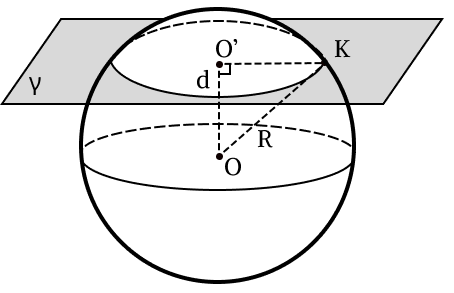
\includegraphics[width=0.2\textwidth]{images/img1}\\
    \end{center}


        \[  O'K =  \sqrt{R ^ 2 - d ^ 2} = \sqrt{(13,5) ^ 2 - (4,5) ^ 2} = \sqrt {9 * 18} = 9\sqrt {2} \text{ см}\]

        \[ L = 2\pi r = 18\sqrt {2} \pi  \text{ см}\]

    Ответ: радиус - $9\sqrt{2}$ см, длина - $18\sqrt {2} \pi$ см

\end{document}
